\documentclass[a4paper, 11pt]{article}
\usepackage{fullpage}
\usepackage{url}
\usepackage{graphicx}
\usepackage{paralist}
\usepackage{wrapfig}
\begin{document}
\title{[DRAFT]\\Customisation of Zombie Riot on\\i3D server \#04 [213.163.69.138:27015]}
\author{Dan ``Chimera'' Cassey}
\begin{figure}
\vspace{-20pt}

\includegraphics[width=4cm]{i3D_logo.pdf}
\vspace{-60pt}
\end{figure}
\maketitle
\section{Introduction}
This document outlines the Specification and Design for the modification to the i3D Zombie Riot server as suggested by Rob.
\section{Background Information: Night of the Dead server}
Rob's suggestions stem from a current server, located in the United States of America, called ``Night of the Dead''. The server runs Zombie Hell mod, the precursor to Zombie Riot, written for EventScripts. The server has been heavily customised, including a human class system, a currency system and player character customisation. Player customisation includes changing the character model, adding motion trails behind the player and adding player glow effects.
\section{Specification}
\begin{enumerate}
\item This project will be in the form of a plug-in for the SourceMod\cite{1} scripting platform, written in SourcePawn and using SQLite for local persistance.
\item This plug-in will be running on a Source Dedicated Server on Linux running Counter-Strike: Source
\item This plug-in will run in parallel with the Zombie Riot mod by Greyscale\cite{2}.
\item This plugin shall implement a human class system with the following classes:
\begin{description}
\item[Assault] Allows the player run faster.
\item[Sniper] Allows the player to cause more damage when using sniper rifles.
\item[Medic] Allows the player to heal team mates.
\item[Support] Gives the player 200\% more bullets per magazine for the M249 light machine gun.
\end{description}
These are the current classes on the Night of the Dead server. We may add further classes in the future as deemed necessary.
\item This plugin shall allow players to customise thier in-game character. This is to be implemented with a !shop menu where players can buy items for thier character and a credit system where players earn credits \begin{inparaenum}[\itshape a\upshape)]\item for in-game events such as joining the server, remaining on the server for a prolonged period of time and getting kills; or \item by selling previously purchased character modifications. \end{inparaenum}
\end{enumerate}

\section{Design}

\subsection{Source Code Structure}
TODO

\subsection{Database}
\begin{wrapfigure}{r}{6cm}
\center
\vspace{-20pt}
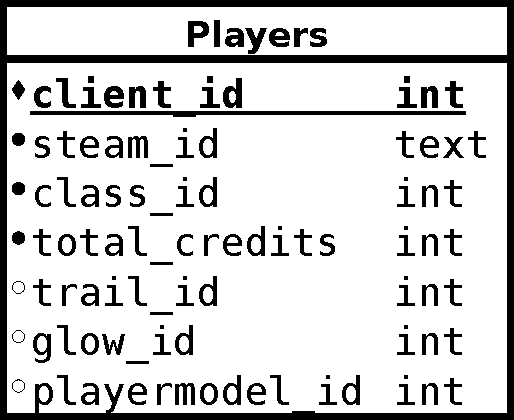
\includegraphics[width=4cm]{Design_Database.pdf}
\vspace{-10pt}
\caption{Design of the single table of the database showing field attributes}
\vspace{-10pt}
\end{wrapfigure}
The database used for persistance will consist of a single table for storing the attributes of individual players. This table will use external integer IDs which will refer to entities defined on configuration key-value files. The diagram shown right details the sqlite table design specification. The primary key, Client ID, should be auto-generated by sqlite but shall not be used by the system. A player will be identified in the table using thier unique Steam ID (in the form STEAM\_0:X:XXXXXXXX where the Xs are integers between 0 and 9). Total credits is the amount of currency, this player can spend on customisations. Class ID, Trail ID, Glow ID, and Playermodel ID are integers that correspond to classes, trails, glows and player models respectively defined in the KV configs.

\subsection{Key-Value (KV) Configuration Files}
The KV config files will allow administator users of the system to define classes and player customisations for their own needs. This system will use 4 KV files: classes, trails, glows and models. When parsing these files, certain conditions need to be met, otherwise the system will log an error and disable the affected module of the system. Example conditions: all identifiers must be unique and non-null, all modifiers must be greater than zero and non-null.

\subsubsection{classes.kv}
The Classes KV will define the identifiers and modifiers of the human classes. Each entry will contain the following fields:
\begin{description}
\item[class\_id]The unique identifier of this class.
\item[class\_name]The name of this class, used for menus and messages.
\item[is\_healer\_class]Bloolean value indicating if this is a medic class.
\item[medic\_medpacks]Number of medpacks available to give in a round. Only applicable when is\_healer\_class is set to true.
\item[modifier\_health]The modifier for the starting health of this class.
\item[modifier\_speed]The modifier for the player speed of this class.
\item[modifier\_damage\_rifle]The modifier for the damage done by assault rifles
\item[modifier\_damage\_sniper]The modifier for the damage done by sniper rifles
\item[modifier\_damage\_lmg]The modifier for the damage done by the light machine gun
\item[modifier\_damage\_smg]The modifier for the damage done by sub machine guns
\item[modifier\_damage\_shotgun]The modifier for the damage done by shotguns
\item[modifier\_bullets\_rifle]The modifier for the number of bullets given to a player when purchasing an assault rifle.
\item[modifier\_bullets\_sniper]The modifier for the number of bullets given to a player when purchasing a sniper rifle.
\item[modifier\_bullets\_lmg]The modifier for the number of bullets given to a player when purchasing the lmg.
\item[modifier\_bullets\_smg]The modifier for the number of bullets given to a player when purchasing a sub machine gun.
\item[modifier\_shells\_shotgun]The modifier for the number of shells given to a player when purchasing a shotgun.
\item[modifier\_magazine\_rifle]The modifier for the size of assault rifle magazines.
\item[modifier\_magazine\_sniper]The modifier for the size of sniper rifle magazines.
\item[modifier\_magazine\_lmg]The modifier for the size of light machine gun magazines.
\item[modifier\_magazine\_smg]The modifier for the size of sub machine gun magazines.
\item[modifier\_magazine\_shotgun]The modifier for the size of shotgun magazines.
\end{description}

\subsubsection{trails.kv}
The Trails KV will define the identifiers and effect files for the trails.
TODO

\subsubsection{glows.kv}
The Glows KV will define the identifiers and effect files for the glows.
TODO

\subsubsection{models.kv}
The Modes KV will define the identifiers and model file paths for the player models.
TODO

\vfill
\begin{thebibliography}{9}
\bibitem{1}
SourceMod: Half-Life 2 Scripting, \url{http://www.sourcemod.net/} [Online], accessed \today.
\bibitem{2}
Zombie Riot - Allied Modders, \url{http://forums.alliedmods.net/showthread.php?p=647040} [Online], accessed \today.
\end{thebibliography}
\begin{figure}[h!]

\includegraphics[width=3cm]{Valve_logo.pdf}
\hfill

\includegraphics[width=3cm]{Counter-Strike_Source_logo.pdf}
\hfill

\includegraphics[width=3cm]{Source_engine_logo.pdf}
\end{figure}
Valve, the Valve logo, Counter-Strike, the Counter-Strike logo, Source and the Source logo are trademarks and/or registered trademarks of Valve Corporation.
\end{document}